% Appendix A

\chapter{Circuitos esquemáticos} % Main appendix title

\label{AppendixA} % For referencing this appendix elsewhere, use \ref{AppendixA}
\pagebreak
\newpage
\begin{figure}[H]
	\centering
	%\includepdf[pages={1}, angle=90]{./Figures/output.driverled.pdf}
	\includegraphics[width=1.66\textwidth, angle=90]{./Figures/output.driverled.pdf}
	\caption{Circuito esquemático de la placa controladora de los carteles de matriz led.}
	\label{fig:schDriverled}
\end{figure}

\begin{figure}[H]
	\centering
	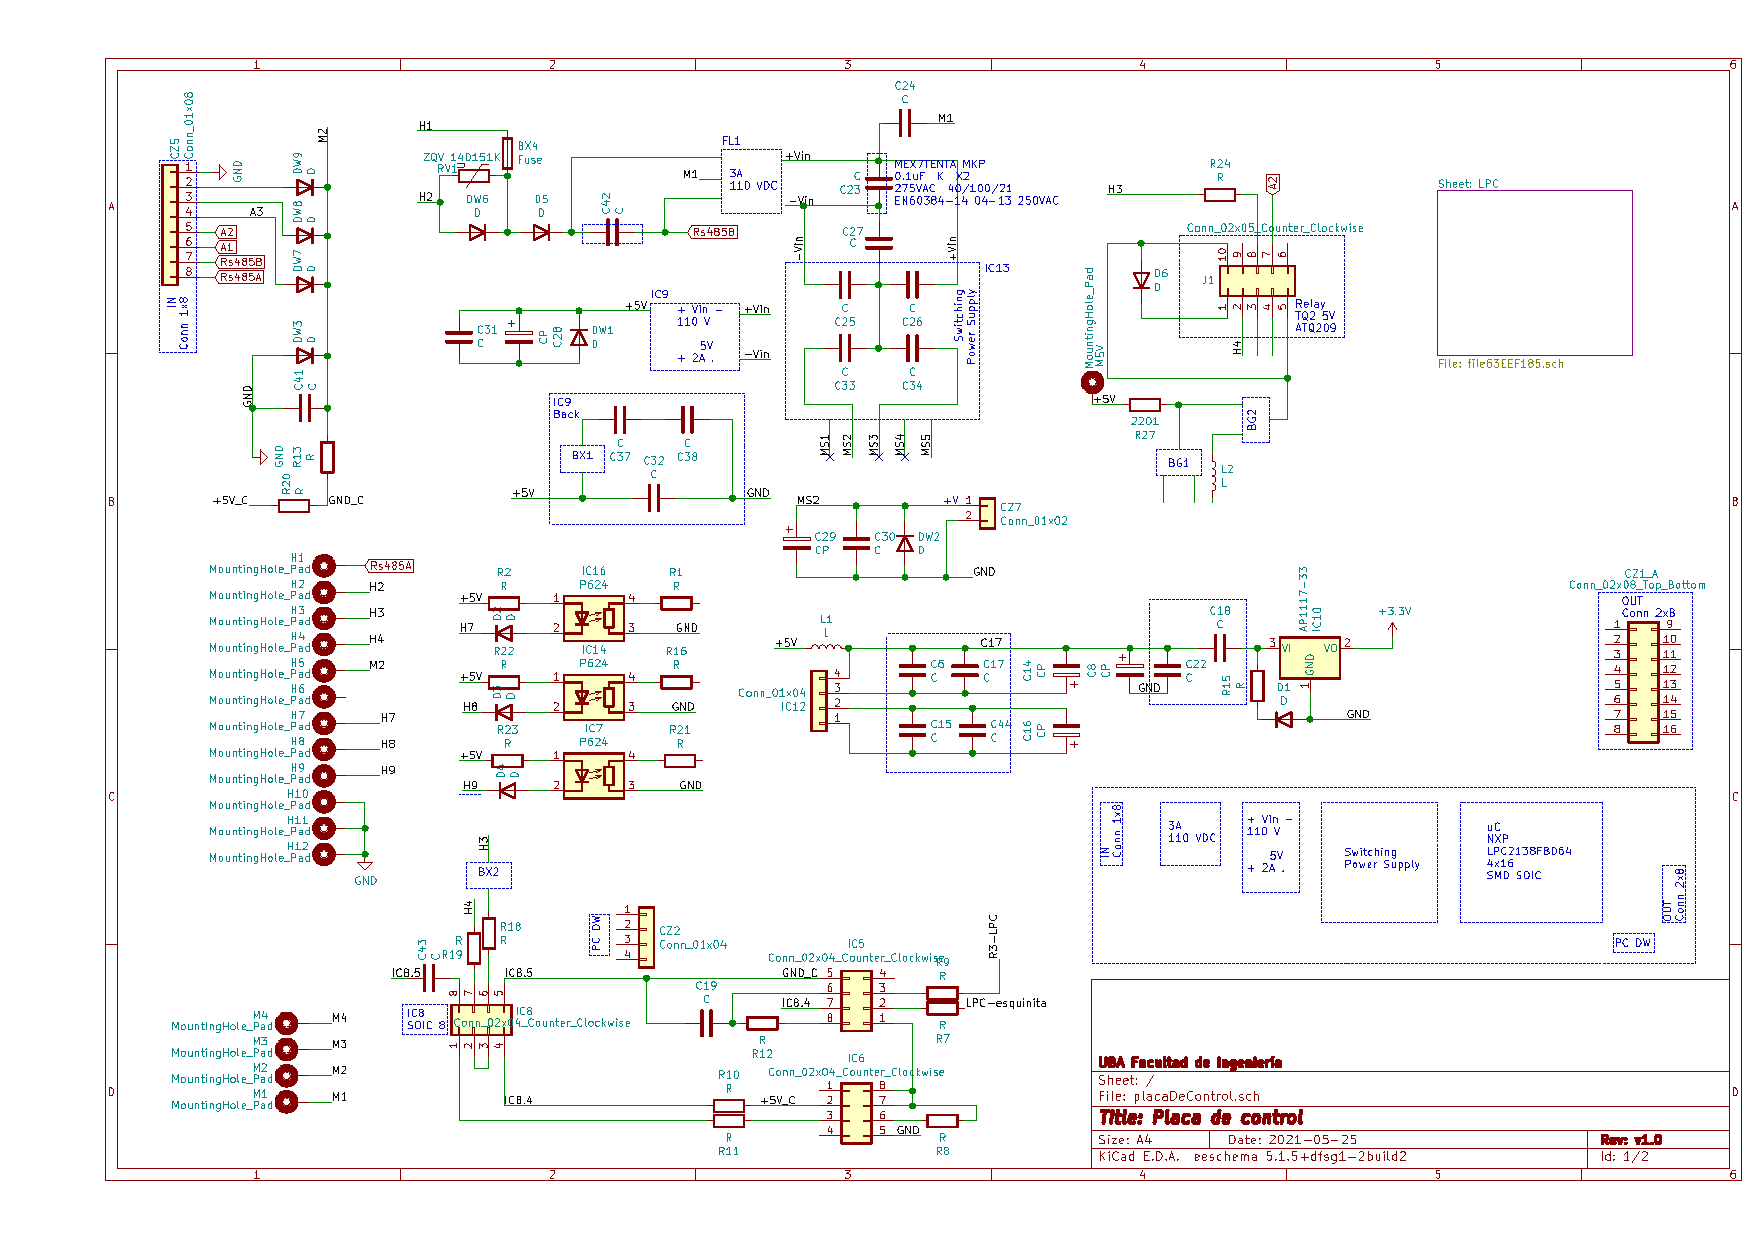
\includegraphics[width=1.66\textwidth, angle=90]{./Figures/output.placaControl.pdf}
	\caption{Circuito esquemático de la placa de control de los carteles LED de salón.}
	\label{fig:schController}
\end{figure}